\documentclass{beamer}

\usetheme{Berkeley}

\graphicspath{{../thesis/graphics/}}
\DeclareGraphicsExtensions{.pdf,.jpeg,.jpg,.png}

\usepackage[utf8]{inputenc}
\usepackage{listings}

\setbeamerfont{frametitle}{family=\rmfamily,series=\bfseries,size={\fontsize{11}{11}}}
\setbeamertemplate{footline}[page number]
\setbeamertemplate{navigation symbols}{} % remove navigation bar

\logo{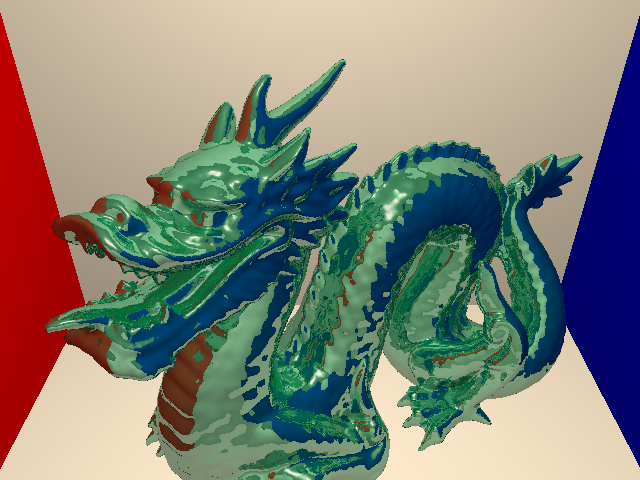
\includegraphics[width=1.5cm, height=1.5cm]{semiReflectingDragon}}
\author{\textsc{Asger Dam Hoedt}}
\title{\textsc{Efficient Ray Tracing of Dynamic Scenes on the GPU}}

\usepackage{algorithmic}
% Algorithm macros
\newcommand{\PARALLELFOR}[2]{\FOR{\textbf{each} #1 \textbf{in} #2 \textbf{in parallel}}}
\newcommand{\FOREACH}[2]{\FOR{\textbf{each} #1 \textbf{in} #2}}
\newcommand{\COMMENTIT}[1]{\STATE{\textit{\color{gray}// #1}}}
\newcommand{\PROCEDURE}[4]{\STATE{\hspace*{-1em}\textbf{procedure} #1 \\ 
    \hspace*{0.5em} \textbf{in} #2 \\ 
    \ifthenelse{\equal{#3}{}}{}{\hspace*{0.5em} \textbf{out} #3 \\}
    \hspace*{-1em}\textbf{begin} \\
    #4 \\
    \hspace*{-1em}\textbf{end}}}
\newcommand{\SYNC}{\STATE{\textbf{synchronize}}}
\newcommand{\ASSIGN}[2]{
  \STATE{#1 $\leftarrow$ #2}
}
\newcommand{\VAR}[1]{$#1$}
\newcommand{\DECLARE}[2]{\STATE{#1 : #2}}
\newcommand{\MIN}[2]{\textbf{min}$($ #1 , #2 $)$}
\newcommand{\MAX}[2]{\textbf{max}$($ #1 , #2 $)$}
\newcommand{\MOD}{\textbf{mod }}

\usepackage{tikz}
\usetikzlibrary{positioning,shadows,arrows}
%Tikz macroes
\tikzset{
  node/.style={rectangle, rounded corners=3mm, fill=white, draw, drop shadow},
%  visitedNode/.style={rectangle, fill=gray!40, draw, drop shadow},
  leaf/.style={rectangle, rounded corners=1mm, fill=white, draw, drop shadow},
%  visitedLeaf/.style={rectangle, rounded corners=1mm, fill=gray!40, draw, drop shadow},
  applyOp/.style={-stealth}
}
\newcommand{\drawTri}[3]{
  \draw[fill=lightgray, drop shadow, rounded corners=0mm] (#1) -- (#2) -- (#3) -- (#1);
}
\newcommand{\drawAabb}[4]{
    \draw[dashed] (#1) -- (#2) -- (#3) -- (#4) -- (#1);
}
\newcommand{\drawRay}[2]{
    \draw[line width=0.5pt, dashed, -stealth] (#1) -- (#2);
}
\newcommand{\drawNode}[4]{
    \draw (#1) -- (#2) -- (#3) -- (#4) -- (#1);
}
\newcommand{\drawSplit}[2]{
  \draw[dashed,line width=0.75pt] (#1) -- (#2);
}
\newcommand{\axes}[2]{
  \draw[->] (0,0) -- coordinate (x axis mid) (#1,0);
  \draw[->] (0,0) -- coordinate (y axis mid) (0,#2);
  %ticks
  \foreach \x in {0,2,...,#1}
            \draw (\x,1pt) -- (\x,-3pt)
		    node[anchor=north] {\x};
  \foreach \y in {0,2,...,#2}
     	    \draw (1pt,\y) -- (-3pt,\y) 
     		    node[anchor=east] {\y}; 

}

\newcommand{\scene}{
  \axes{11}{9}

  % Tris
  \drawTri{0,6}{2,8}{2,4}
  \draw (1.33,6.5) node {0};
  \drawTri{2,6}{4,8}{2,8}
  \draw (2.66,7.33) node {1};
  \drawTri{2,6}{4,4}{2,4}
  \draw (2.67,4.67) node {3};

  \drawTri{7,8}{7,4}{9,4}
  \draw (7.67,5.33) node {2};
  \drawTri{9,0}{10,2}{6,3}
  \draw (8.33,1.66) node {4};
  \drawTri{6,3}{6,1}{8,1}
  \draw (6.67,1.67) node {5};
}

\newcommand{\sceneAabb}{
  \drawAabb{0,4}{0,8}{2,8}{2,4}
  \drawAabb{2,4}{2,6}{4,6}{4,4}
  \drawAabb{2,6}{2,8}{4,8}{4,6}
  \drawAabb{7,4}{7,8}{9,8}{9,4}
  \drawAabb{6,0}{6,3}{10,3}{10,0}
  \drawAabb{6,1}{6,3}{8,3}{8,1}
}

\begin{document}

%\tiny

\begin{frame}
  \begin{center}
    \frametitle{Efficient Ray Tracing of Dynamic Scenes on the GPU}
    \footnotesize
    Master's Thesis Exam - April 28, 2011 - Aarhus University
    \vspace*{15pt}\\
    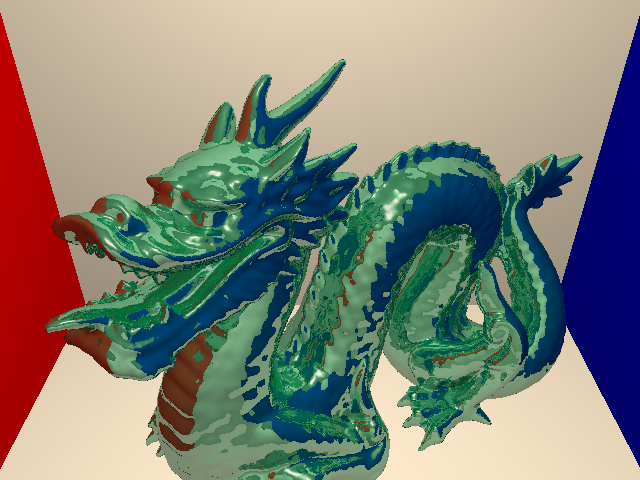
\includegraphics[width=6cm]{semiReflectingDragon}
    \vspace*{20pt}
    \\
    \begin{minipage}{0.4\textwidth}
      \centering
      Asger Dam Hoedt \\ asgerhoedt@gmail.com \\ 20051770
    \end{minipage}
    \begin{minipage}{0.4\textwidth}
      \centering
      Thomas Sangild Sørensen \\ sangild@cs.au.dk \\ Supervisor
    \end{minipage}
  \end{center}
\end{frame}

\section{Introduction}
\begin{frame}
  \frametitle{Motivation and Goals}

  Motivation
  \begin{itemize}
  \item Increasing interest in ray tracing for creating photo realistic images.
  \item Usecases include CGI effects in modern films, CAD rendering and lighting
    in games.
  \end{itemize}

  Goals
  \begin{itemize}
    \item Minimize the time betwen modifying a scene and presenting visual
      feedback.
    \item Achieve this by examining the relationship between tree quality and
      construction time.
    \item GPU implementation to exploit the massive computational power of
      todays graphics cards.
  \end{itemize}
\end{frame}

%% \begin{frame}
%%   \frametitle{Domain}
%%   \begin{itemize}
%%   \item Use KD-tree to accelerate ray tracing.
%%   \item GPU implementation to utilize the massive computational power of today's
%%     graphics hardware.
%%   \end{itemize}
%% \end{frame}

%% \begin{frame}
%%   \frametitle{Goals}
%%   \begin{itemize}
%%     \item Minimize the time betwen modifying a scene and presenting visual
%%       feedback.
%%     \item Achieve this by examining the relationship between tree quality and
%%       construction time.
%%   \end{itemize}
%% \end{frame}

\section{KD-Trees}
\begin{frame}
  \frametitle{KD-Trees}

  \begin{itemize}
    \item Exhaustive ray tracing is too expensive.
    \item Introduce hierarchical data structures to spatially subdivide scenes.
    \item I chose KD-trees and based it on the paper by Zhou et al.
  \end{itemize}
\end{frame}

\subsection{Example}
\begin{frame}
  \frametitle{Example Scene}
  \begin{minipage}{0.4\textwidth}
    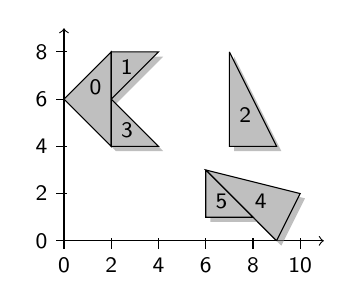
\begin{tikzpicture}[y=0.3cm, x=.3cm,font=\sffamily]
      \footnotesize
      \scene
    \end{tikzpicture}
  \end{minipage}
  \begin{minipage}{0.5\textwidth}
    \centering
    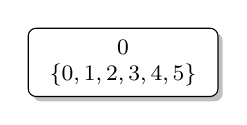
\begin{tikzpicture}[y=0.3cm, x=.3cm,font=\sffamily]
      \footnotesize
      \node [leaf] {$\begin{array}{c}0\\\{0,1,2,3,4,5\}\end{array}$};
    \end{tikzpicture}
  \end{minipage}
\end{frame}

\begin{frame}
  \frametitle{First level split}
  \begin{minipage}{0.4\textwidth}
    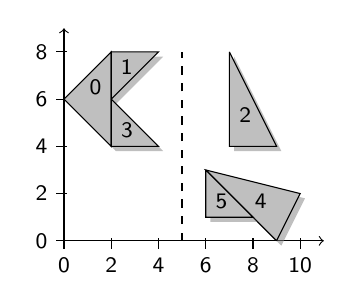
\begin{tikzpicture}[y=0.3cm, x=.3cm,font=\sffamily]
      \footnotesize
      \scene
      
      % splits
      \drawSplit{5,0}{5,8}
    \end{tikzpicture}
  \end{minipage}
  \begin{minipage}{0.5\textwidth}
    \centering
    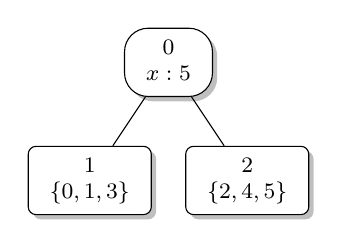
\begin{tikzpicture}[y=0.3cm, x=.3cm,font=\sffamily,
        level 1/.style={sibling distance=20mm}]
      \footnotesize
      \node [node] {$\begin{array}{c}0\\x:5\end{array}$}
        child {node [leaf] {$\begin{array}{c}1\\\{0,1,3\}\end{array}$}}
        child {node [leaf] {$\begin{array}{c}2\\\{2,4,5\}\end{array}$}};
    \end{tikzpicture}
  \end{minipage}
\end{frame}

\begin{frame}
  \frametitle{Second level splits}
  \begin{minipage}{0.4\textwidth}
    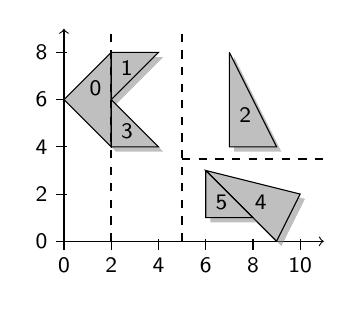
\begin{tikzpicture}[y=0.3cm, x=.3cm,font=\sffamily]
      \footnotesize
      \scene
      
      % splits
      \drawSplit{5,0}{5,9}
      \drawSplit{2,0}{2,9}
      \drawSplit{5,3.5}{11,3.5}
    \end{tikzpicture}
  \end{minipage}
  \begin{minipage}{0.5\textwidth}
    \centering
    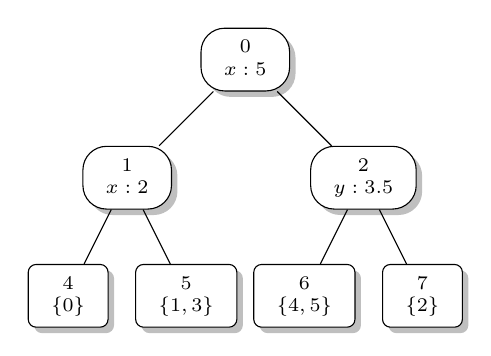
\begin{tikzpicture}[y=0.3cm, x=.3cm,font={\sffamily\scriptsize},
        level 1/.style={sibling distance=30mm}, 
        level 2/.style={sibling distance=15mm}]
      \node [node] {$\begin{array}{c}0\\x:5\end{array}$}
        child {node [node] {$\begin{array}{c}1\\x:2\end{array}$}
          child {node [leaf] {$\begin{array}{c}4\\\{0\}\end{array}$}}
          child {node [leaf] {$\begin{array}{c}5\\\{1,3\}\end{array}$}}}
        child {node [node] {$\begin{array}{c}2\\y:3.5\end{array}$}
          child {node [leaf] {$\begin{array}{c}6\\\{4,5\}\end{array}$}}
          child {node [leaf] {$\begin{array}{c}7\\\{2\}\end{array}$}}};
    \end{tikzpicture}
  \end{minipage}

  Note to self: All the brilliance in costructing kd-trees comes down to where
  to place the splitting plane and how to associate primitives with new nodes.

\end{frame}


\subsection{Memory Representation}
\begin{frame}
  \frametitle{Memory Representation}
  \begin{itemize}
  \item How to represent interior nodes and leaf nodes?
  \item How to place the nodes in memory?
  \end{itemize}
\end{frame}

\subsubsection{Node representations}
\begin{frame}[fragile]
  \frametitle{Interior Node Representation}
  An interior node must contain:
  \begin{itemize}
  \item \textit{Split axis} - The axis that an interior node is split
    along.
  \item \textit{Split position} - The position of the splitting plane
    along the split axis.
  \item \textit{Child references} - Information about how to find the
    node's children.
  \end{itemize}

  \begin{lstlisting}[language=C++]
struct KDInterior {
  char axis; // {X, Y, Z}
  float splitPosition;
  KDNode *left, *right;
};
  \end{lstlisting}
\end{frame}

\begin{frame}[fragile]
  \frametitle{Leaf Node Representation}
  A leaf node must contain:
  \begin{itemize}
    \item \textit{Associated triangles} - A representation of the triangles
      associated with the leaf node.
  \end{itemize}
  \begin{lstlisting}[language=C++]
struct KDLeaf {
  int triangleIndex, triangleRange;
};
  \end{lstlisting}
\end{frame}

\begin{frame}[fragile]
  \frametitle{Node Representation}
  \begin{itemize}
  \item The complete KDNode is combination of the two node types.
  \end{itemize}
  
  \begin{lstlisting}[language=C++]
struct KDNode {
  char nodeType; // {Child, X, Y, Z}
  float splitPosition;
  KDNode *left, *right;
  int triangleIndex, triangleRange;
};
  \end{lstlisting}
\end{frame}


\subsubsection{Memory Layout}
\begin{frame}
  \frametitle{Memory Layout}

  \begin{itemize}
  \item The nodes are placed in memory in a linear array.
    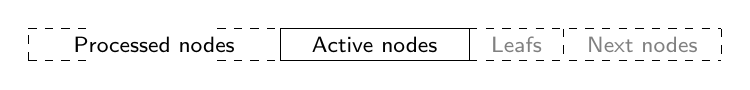
\begin{tikzpicture}[y=0.4cm, x=0.4cm,font={\sffamily\footnotesize}]
      
      \draw[dashed] (0,1) -- (2,1);
      \draw[dashed] (0,0) -- (0,1);
      \draw[dashed] (0,0) -- (2,0);
      \draw (4,0.5) node {Processed nodes};
      \draw[dashed] (6,1) -- (8,1);
      \draw[dashed] (6,0) -- (8,0);
      \draw (8,1) -- (8,0);
      
      \draw (8,1) -- (14,1);
      \draw (8,0) -- (14,0);
    
      \draw (11,0.5) node {Active nodes};
      \draw (14,1) -- (14,0);
      
      \draw[dashed] (14,1) -- (22,1);
      \draw[dashed] (14,0) -- (22,0);

      \draw (15.5,0.5) node {\color{gray}Leafs};
      \draw[dashed] (17,1) -- (17,0);
      
      \draw (19.5,0.5) node {\color{gray}Next nodes};
      \draw[dashed] (22,1) -- (22,0);
      
    \end{tikzpicture}
    
  \item This structure allows for coallesced access to the nodes currently being
    processed.
  \item Data is stored as a struct of arrays instead of arrays of structs.
  \item Geometrix primitives are also stored in a linear array
  \end{itemize}
\end{frame}

\subsection{Construction}
\begin{frame}
  \frametitle{Construction}
  
  \begin{itemize}
    \item Must take full advantage of the GPU's data parallel architecture!
    \item Use breath-first construction instead of depth-first.
    \item Split construction into 2 phases; One for the upper nodes and one for
      the lower.
  \end{itemize}
\end{frame}

\subsubsection{Upper Nodes}
\begin{frame}
  \frametitle{Upper Node Construction}
  
  \begin{itemize}
  \item Construct in breath-first order.
  \item Parallize over all primitives.
  \item Use spatial median splitting to place splitting planes.
  \item Improve tree quality by adding Empty Space Maximization.
  \end{itemize}
\end{frame}

\begin{frame}
  \frametitle{Upper Node Construction Algorithm}
  
  \begin{algorithmic}
    \scriptsize
    \PROCEDURE{CreateNodes}
              {$activeNodes$ : Node List}
              {$leafNodes, nextNodes$ : Node List}
              {\PARALLELFOR{$n$}{$activeNodes$}
                  \STATE{Determine $n$'s splitting plane using spatial median splitting.}
                \ENDFOR
                \PARALLELFOR{$p$}{$primitives$}
                  \STATE{Sort $p$ to its new position to maintain
                    node/prim association.}
                \ENDFOR
                \PARALLELFOR{$n$}{$activeNodes$}
                  \STATE{Create $n$'s children and store in $leafNodes$ and $nextNodes$.}
                \ENDFOR}
  \end{algorithmic}
  
\end{frame}

\begin{frame}
  \frametitle{Upper Node Example: Initial primitives}

  \begin{itemize}
  \item First calculate axis aligned bounding volumes for the geometry.
  \end{itemize}
  
  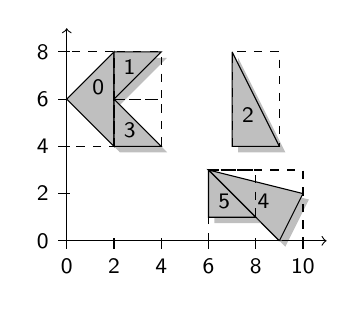
\begin{tikzpicture}[y=0.3cm, x=.3cm,font={\sffamily\footnotesize}]
    \scene
    \sceneAabb
  \end{tikzpicture}

  \begin{itemize}
  \item $primitive \leftarrow [t_0,t_1,t_2,t_3,t_4,t_5]$
  \item $primAabbMin \leftarrow [(0,4),(2,6),(7,4),(2,4),(6,0),(6,1)]$
  \item $primAabbMax \leftarrow [(2,8),(4,8),(9,8),(4,6),(10,3),(8,3)]$
  \end{itemize}
  
\end{frame}

\begin{frame}
  \frametitle{Upper Node Example: Root Node}
  
  \begin{itemize}
    \item Initialize the root node.
    \item $nodes[0] \leftarrow KDLeaf($CHILD$, 0, primitives)$
  \end{itemize}

\end{frame}

\begin{frame}[fragile]
  \frametitle{Upper Node Example: Segments}
  \begin{itemize}
  \item Partition the active nodes into segments of up to 2 primitives per
    segment.\\
  \begin{lstlisting}[language=C++]
struct Segment {
  int owner; // Associated interior node
  int index, range;
};
    \end{lstlisting}

   $\begin{array}{lccc}
    owner: & n_0 & n_0 & n_0\\
    index: & 0 & 2 & 4\\
    range: & 2 & 2 & 2\\
  \end{array}$
  \end{itemize}
\end{frame}

\begin{frame}
  \frametitle{Upper Node Example: Position Split Plane}
  
  \begin{itemize}
    \item Compute segments AABB in parallel.\\
      $\begin{array}{lccc}
      owner: & n_0 & n_0 & 0\\
      min: & (0,4) & (2,4) & (6,0)\\
      max: & (4,8) & (9,8) & (10,3)\\
    \end{array}$
    \item Reduce $min$ and $max$ to owner node in parallel.\\
      $\begin{array}{lc}
      node: & n_0 \\
      min: & (0,0)\\
      max: & (10,8)\\
    \end{array}$
    \item Place splitting plane at the spatial median of the largest axis (in
      parallel).\\
      $\begin{array}{lc}
      node: & n_0 \\
      type: & X\\
      position: & 5\\
    \end{array}$
  \end{itemize}
\end{frame}

\begin{frame}
  \frametitle{Upper Node Example: Sort primitives}
  
  \begin{itemize}
  \item Sort primitives according to their associated nodes splitting plane.
  \item Flag which side of the plane the primitives belong to.\\
    $\begin{array}{lcccccc}
    primitive: & t_0 & t_1 & t_2 & t_3 & t_4 & t_5 \\
    left:  & 1 & 1 & 0 & 1 & 0 & 0 \\
    right: & 0 & 0 & 1 & 0 & 1 & 1 \\
    \end{array}$
  \item Compute where to sort the primitives to.\\
    $\begin{array}{lccccccccccccc}
    left+right: & 1 & 1 & 0 & 1 & 0 & 0 & 0 & 0 & 1 & 0 & 1 & 1 \\
    address:    & 0 & 1 & 2 & 2 & 3 & 3 & 3 & 3 & 3 & 4 & 4 & 5 & 6\\
    \end{array}$
  \item Finally sort the primitives.\\
    $primitives: [t_0, t_1, t_3, t_2, t_4, t_5]$
  \end{itemize}
\end{frame}

\begin{frame}
  \frametitle{Upper Node Example: Construct new leaf nodes}
  \begin{itemize}
    \item Compute the index and range of the new leaf nodes in parallel using $address$.\\
      $\begin{array}{lcc}
      child: & n_0.left & n_0.right \\
      index: & 0 & 3 \\
      range: & 3 & 3 \\
      \end{array}$
    \item Compute their location in the list of nodes in parallel\\
      $\begin{array}{lcc}
      child: & n_0.left & n_0.right \\
      address: & 1 & 2 \\
      \end{array}$
    \item Create the new nodes as leaf nodes.\\
      $\begin{array}{lcc}
      node: & n_1 & n_2\\
      index: & 0 & 3\\
      range: & 3 & 3\\
      \end{array}$
  \end{itemize}
\end{frame}

\begin{frame}
  \frametitle{Upper Node Example: First Iteration}
  \begin{minipage}{0.4\textwidth}
    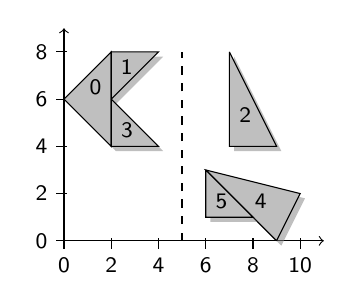
\begin{tikzpicture}[y=0.3cm, x=.3cm,font=\sffamily]
      \footnotesize
      \scene
      
      % splits
      \drawSplit{5,0}{5,8}
    \end{tikzpicture}
  \end{minipage}
  \begin{minipage}{0.5\textwidth}
    \centering
    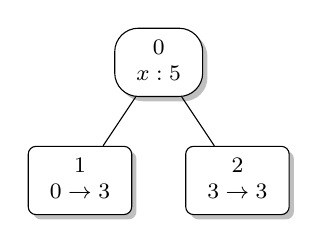
\begin{tikzpicture}[y=0.3cm, x=.3cm,font=\sffamily,
        level 1/.style={sibling distance=20mm}]
      \footnotesize
      \node [node] {$\begin{array}{c}0\\x:5\end{array}$}
        child {node [leaf] {$\begin{array}{c}1\\0 \rightarrow 3\end{array}$}}
        child {node [leaf] {$\begin{array}{c}2\\3 \rightarrow 3\end{array}$}};
    \end{tikzpicture}
  \end{minipage}
  \vspace{10pt}
  \begin{itemize}
    \item[] $primitives: t_0, t_1, t_3, t_2, t_4, t_5$
  \end{itemize}
\end{frame}

\begin{frame}
  \frametitle{Upper Node Example: Segments}
  \begin{itemize}
  \item Partition the active nodes into segments of up to 2 primitives per
    segment.\\
    $\begin{array}{lcccc}
      owner: & n_1 & n_1 & n_2 & n_2 \\
      index: & 0 & 2 & 3 & 5 \\
      range: & 2 & 1 & 2 & 1 \\
    \end{array}$
  \end{itemize}
\end{frame}

\begin{frame}
  \frametitle{Upper Node Example: Position Split Plane}
  \begin{itemize}
    \item Compute segments AABB in parallel.\\
      $\begin{array}{lcccc}
      owner: & n_1 & n_1 & n_2 & n_2 \\
      min: & (0,4) & (2,4) & (6,0) & (6,1)\\
      max: & (4,8) & (4,6) & (10,8) & (8,3)\\
    \end{array}$
    \item Reduce $min$ and $max$ to owner node in parallel.\\
      $\begin{array}{lcc}
      node: & n_1 & n_2 \\
      min: & (0,4) & (6,0) \\
      max: & (4,8) & (10,8) \\
    \end{array}$
    \item Place splitting plane at the spatial median of the largest axis in
      parallel.\\
      $\begin{array}{lcc}
        node: & n_1 & n_2 \\
        type: & Y & Y \\
        position: & 6 & 4 \\
      \end{array}$
  \end{itemize}
\end{frame}

\begin{frame}
  \frametitle{Upper Node Example: Sort primitives}
  
  \begin{itemize}
  \item Flag which side of the plane the primitives belong to.\\
    $\begin{array}{lcccccc}
      primitive: & t_0 & t_1 & t_3 & t_2 & t_4 & t_5 \\
      left:  & 1 & 0 & 1 & 0 & 1 & 1 \\
      right: & 1 & 1 & 0 & 1 & 0 & 0 \\
    \end{array}$
  \item Compute where to sort the primitives to.\\
    $\begin{array}{lccccccccccccc}
%     left+right: & 0 & 1 & 3 & 2 & 4 & 5 & 0 & 1 & 3 & 2 & 4 & 5 \\
      left+right: & 1 & 0 & 1 & 0 & 1 & 1 & 1 & 1 & 0 & 1 & 0 & 0 \\
      address:    & 0 & 1 & 1 & 2 & 2 & 3 & 4 & 5 & 6 & 6 & 7 & 7 & 7 \\
    \end{array}$
  \item Finally sort the primitives.\\
    $primitives: t_0, t_3, t_4, t_5, t_0, t_1, t_2$
  \end{itemize}
\end{frame}

\begin{frame}
  \frametitle{Upper Node Example: Construct new leaf nodes}
  \begin{itemize}
    \item Compute the index and range of the new leaf nodes in parallel using
      $address$.\\
      $\begin{array}{lcccc}
        child: & n_1.left & n_1.right & n_2.left & n_2.right \\
        index: & 0 & 4 & 2 & 6 \\
        range: & 2 & 2 & 2 & 1 \\
      \end{array}$
    \item Compute their location in the list of nodes in parallel\\
      $\begin{array}{lcccc}
        child: & n_1.left & n_1.right & n_2.left & n_2.right \\
        address: & 3 & 4 & 5 & 6 \\
      \end{array}$
    \item Create the new nodes as leaf nodes.\\
  \end{itemize}
\end{frame}

\begin{frame}
  \frametitle{Upper Node Example: Second Iteration}
  \begin{minipage}{0.4\textwidth}
    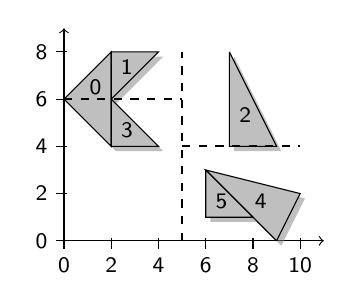
\begin{tikzpicture}[y=0.3cm, x=.3cm,font=\sffamily]
      \footnotesize
      \scene
      
      % splits
      \drawSplit{5,0}{5,8}
      \drawSplit{0,6}{5,6}
      \drawSplit{5,4}{10,4}
    \end{tikzpicture}
  \end{minipage}
  \begin{minipage}{0.5\textwidth}
    \centering
    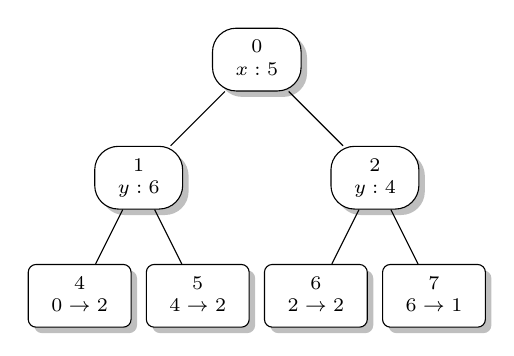
\begin{tikzpicture}[y=0.3cm, x=.3cm,font={\sffamily\scriptsize},
        level 1/.style={sibling distance=30mm}, 
        level 2/.style={sibling distance=15mm}]
      \node [node] {$\begin{array}{c}0\\x:5\end{array}$}
        child {node [node] {$\begin{array}{c}1\\y:6\end{array}$}
          child {node [leaf] {$\begin{array}{c}4\\0 \rightarrow 2\end{array}$}}
          child {node [leaf] {$\begin{array}{c}5\\4 \rightarrow 2\end{array}$}}}
        child {node [node] {$\begin{array}{c}2\\y:4\end{array}$}
          child {node [leaf] {$\begin{array}{c}6\\2 \rightarrow 2\end{array}$}}
          child {node [leaf] {$\begin{array}{c}7\\6 \rightarrow 1\end{array}$}}};
    \end{tikzpicture}
  \end{minipage}
  \vspace{10pt}
  \begin{itemize}
    \item[] $primitives: t_0, t_3, t_4, t_5, t_0, t_1, t_2$
  \end{itemize}
\end{frame}

\subsubsection{Empty Space Maximization}
\begin{frame}
  \frametitle{Empty Space Maximization}
  \begin{itemize}
  \item Improves the quality of the constructed tree by adding ``early out''
    empty leafs.
  \item Increases construction time due to extra processing of each tree node.
  \item Must be implemented as a plugable solution for testing purposes.
  \item Empty Space nodes are injected between the active nodes and leaf nodes.
    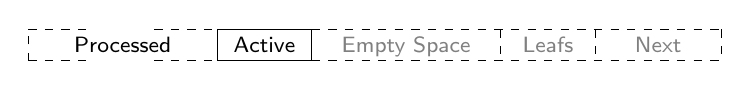
\begin{tikzpicture}[y=0.4cm, x=0.4cm,font={\sffamily\footnotesize}]
      
      \draw[dashed] (0,1) -- (2,1);
      \draw[dashed] (0,0) -- (0,1);
      \draw[dashed] (0,0) -- (2,0);
      \draw (3,0.5) node {Processed};
      \draw[dashed] (4,1) -- (6,1);
      \draw[dashed] (4,0) -- (6,0);
      \draw (6,1) -- (6,0);
      
      \draw (6,1) -- (9,1);
      \draw (6,0) -- (9,0);
    
      \draw (7.5,0.5) node {Active};
      \draw (9,1) -- (9,0);
      
      \draw[dashed] (9,1) -- (22,1);
      \draw[dashed] (9,0) -- (22,0);

      \draw (12,0.45) node {\color{gray}Empty Space};
      \draw[dashed] (15,1) -- (15,0);

      \draw (16.5,0.5) node {\color{gray}Leafs};
      \draw[dashed] (18,1) -- (18,0);
      
      \draw (20,0.5) node {\color{gray}Next};
      \draw[dashed] (22,1) -- (22,0);
      
    \end{tikzpicture}
  \end{itemize}
\end{frame}

\begin{frame}
  \frametitle{Empty Space Maximization}

  \begin{itemize}
  \item Compute new empty space nodes for each active node in parallel.
  \item Use scan to compute address of empty space nodes.
  \item Create nodes.
  \end{itemize}
\end{frame}

\begin{frame}
  \frametitle{Empty Space Maximization Example}
  \begin{minipage}{0.4\textwidth}
    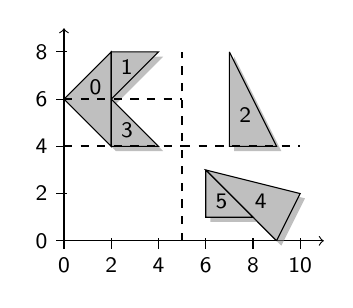
\begin{tikzpicture}[y=0.3cm, x=.3cm,font=\sffamily]
      \footnotesize
      \scene
      
      % splits
      \drawSplit{5,0}{5,8}
      \drawSplit{0,6}{5,6}
      \drawSplit{0,4}{5,4}
      \drawSplit{5,4}{10,4}
    \end{tikzpicture}
  \end{minipage}
  \begin{minipage}{0.5\textwidth}
    \centering
    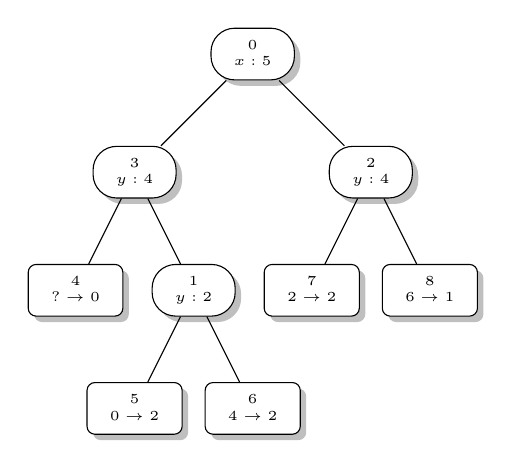
\begin{tikzpicture}[y=0.3cm, x=.3cm,font={\sffamily\tiny},
        level 1/.style={sibling distance=30mm}, 
        level 2/.style={sibling distance=15mm}]
      \node [node] {$\begin{array}{c}0\\x:5\end{array}$}
        child {node [node] {$\begin{array}{c}3\\y:4\end{array}$}
          child {node [leaf] {$\begin{array}{c}4\\? \rightarrow 0\end{array}$}}
          child {node [node] {$\begin{array}{c}1\\y:2\end{array}$}
            child {node [leaf] {$\begin{array}{c}5\\0 \rightarrow 2\end{array}$}}
            child {node [leaf] {$\begin{array}{c}6\\4 \rightarrow 2\end{array}$}}}}
        child {node [node] {$\begin{array}{c}2\\y:4\end{array}$}
          child {node [leaf] {$\begin{array}{c}7\\2 \rightarrow 2\end{array}$}}
          child {node [leaf] {$\begin{array}{c}8\\6 \rightarrow 1\end{array}$}}};
    \end{tikzpicture}
  \end{minipage}
  \vspace{10pt}
  \begin{itemize}
    \item[] $primitives: t_0, t_3, t_4, t_5, t_0, t_1, t_2$
  \end{itemize}
\end{frame}

\subsubsection{Lower Nodes}
\begin{frame}
  \frametitle{Lower Nodes}
  \begin{itemize}
    \item Few primitives per node, but thousands of nodes.
    \item Trivial to implement compared to upper nodes phase.
    \item Favor large leaf nodes.
  \end{itemize}
\end{frame}


\section{Results}
\begin{frame}
  \frametitle{Results}

  \begin{itemize}
    \item Empty Space Maximization ratio
    \item Node association algorithm
  \end{itemize}
\end{frame}

\end{document}
